% bei Standalone in documentclass noch:
% \RequirePackage{luatex85}

\documentclass[captions=tableheading, titlepage= firstiscover, parskip = half , bibliography=totoc]{scrartcl}
%paper = a5 für andere optinen
% titlepage= firstiscover
% bibliography=totoc für bibdateien
% parskip=half  Veränderung um Absätze zu verbessern

\usepackage{scrhack} % nach \documentclass
\usepackage[aux]{rerunfilecheck}
\usepackage{polyglossia}
\usepackage[style=numeric, backend=biber]{biblatex} % mit [style = alphabetic oder numeric] nach polyglossia
\addbibresource{lit.bib}
\setmainlanguage{german}

\usepackage[autostyle]{csquotes}
\usepackage{amsmath} % unverzichtbare Mathe-Befehle
\usepackage{amssymb} % viele Mathe-Symbole
\usepackage{mathtools} % Erweiterungen für amsmath
\usepackage{fontspec} % nach amssymb
% muss ins document: \usefonttheme{professionalfonts} % für Beamer Präsentationen
\usepackage{longtable}

\usepackage[
math-style=ISO,    % \
bold-style=ISO,    % |
sans-style=italic, % | ISO-Standard folgen
nabla=upright,     % |
partial=upright,   % /
]{unicode-math} % "Does exactly what it says on the tin."
\setmathfont{Latin Modern Math}
% \setmathfont{Tex Gyre Pagella Math} % alternativ

\usepackage[
% die folgenden 3 nur einschalten bei documenten
locale=DE,
separate-uncertainty=true, % Immer Fehler mit ±
per-mode=symbol-or-fraction, % m/s im Text, sonst \frac
]{siunitx}

% alternativ:
% per-mode=reciprocal, % m s^{-1}
% output-decimal-marker=., % . statt , für Dezimalzahlen

\usepackage[
version=4,
math-greek=default,
text-greek=default,
]{mhchem}

\usepackage[section, below]{placeins}
\usepackage{caption} % Captions schöner machen
\usepackage{graphicx}
\usepackage{grffile}
\usepackage{subcaption}

% \usepackage{showframe} Wenn man die Ramen sehen will

\usepackage{float}
\floatplacement{figure}{htbp}
\floatplacement{table}{htbp}

\usepackage{mhchem} %chemische Symbole Beispiel: \ce{^{227}_{90}Th+}


\usepackage{booktabs}

 \usepackage{microtype}
 \usepackage{xfrac}

 \usepackage{expl3}
 \usepackage{xparse}

 % \ExplSyntaxOn
 % \NewDocumentComman \I {}  %Befehl\I definieren, keine Argumente
 % {
 %    \symup{i}              %Ergebnis von \I
 % }
 % \ExplSyntaxOff

 \usepackage{pdflscape}
 \usepackage{mleftright}

 % Mit dem mathtools-Befehl \DeclarePairedDelimiter können Befehle erzeugen werden,
 % die Symbole um Ausdrücke setzen.
 % \DeclarePairedDelimiter{\abs}{\lvert}{\rvert}
 % \DeclarePairedDelimiter{\norm}{\lVert}{\rVert}
 % in Mathe:
 %\abs{x} \abs*{\frac{1}{x}}
 %\norm{\symbf{y}}

 % Für Physik IV und Quantenmechanik
 \DeclarePairedDelimiter{\bra}{\langle}{\rvert}
 \DeclarePairedDelimiter{\ket}{\lvert}{\rangle}
 % <name> <#arguments> <left> <right> <body>
 \DeclarePairedDelimiterX{\braket}[2]{\langle}{\rangle}{
 #1 \delimsize| #2
 }

\setlength{\delimitershortfall}{-1sp}

 \usepackage{tikz}
 \usepackage{tikz-feynman}

 \usepackage{csvsimple}
 % Tabellen mit \csvautobooktabular{"file"}
 % muss in table umgebung gesetzt werden


% \multicolumn{#Spalten}{Ausrichtung}{Inhalt}

\usepackage{hyperref}
\usepackage{bookmark}
\usepackage[shortcuts]{extdash} %nach hyperref, bookmark

\newcommand{\ua}[1]{_\symup{#1}}
\newcommand{\su}[1]{\symup{#1}}


\title{Versuch 703}
\subtitle{Das Geiger-Müller-Zählrohr}
\author{Jonah Nitschke\\
        lejonah@web.de \and
        Sebastian Pape\\
        sepa@gmx.de}
\date{Durchführung: 25.04.2017\\
      Abgabe: 02.05.2017}


\begin{document}

\maketitle

\section{Theorie}

\subsection{Zielsetzung}

Mithilfe des Geiger-Müller-Zählrohrs kann in der Kernphysik die Intensität von
ionisierter Strahlung zu messen. Bei dem folgenden Versuch geht es nun darum,
die Funktionsweise eines Geiger-Müller-Zählrohrs durch verschiedene Messungen
zu charakterisieren und die Kerndaten des vorliegenden Geräts zu ermitteln.

\subsection{Aufbau und Wirkungsweise}

Das Geiger-Müller-Zählrohr besteht im Wesentlichen aus einem Kathodenzylinder
mit einerm axial verlaufenden Anodendraht (siehe Abb. \ref{fig:Geiger}). Um die
später genauer beschriebenen Nachentladungseffekte gering zu halten, ist das
Zählrohr zusätzlich mit einem Alkoholgehaltigen Gasgemisch gefüllt. Wird eine
äußere Spannung angelegt, so entsteht zwischen Kathode und Anode ein
radialsymmetrisches Feld. Dringt nun ein Teilchen in das Zählrohrvolumen ein,
so werden abhängig von der angelegten Spannung nach der Primäriosation
verschiedene Effekte hervorgerufen (siehe Abb. \ref{fig:Bereiche}).

\begin{figure}
  \centering
  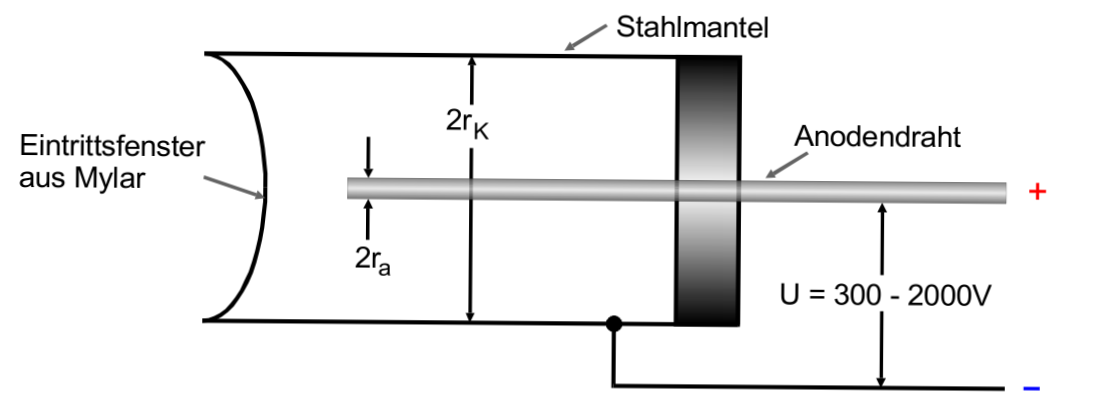
\includegraphics[width=\textwidth]{Zaehlrohr.png}
  \caption{Aufbau des Geiger-Müller-Zählrohrs.}
  \label{fig:Geiger}
\end{figure}

Bei einer sehr geringen Spannung gelangen durch Rekombination bedingt nur sehr
wenige Elektroden an die Anode (Bereich I, Abb. \ref{fig:Bereiche}). Wird die
angelegte Spannung weiter erhöht, gelangen aufgrund der höheren Feldstärke nahezu
alle Elektronen an die Anode und die Rekombinationswahrscheinlichkeit nimmt
stark ab. In diesem als Ionisationskammer (Bereich II, Abb. \ref{fig:Bereiche})
bezeichneten Bereich ist der Ionisationsstrom proportional zu Energie bzw.
Intensität der einfallenden Strahlung.

Bei einer weiteren Erhöhung der Feldstärke können die freigesetzten Elektronen
genügend Energie aufnehmen um ihrerseits ionisieren zu können. Bei einer hinreichend
hohen angelegten Spannung wird durch die Stoßionisation die Zahl der freigesetzten
Elektronen stark erhöht, dieser Vorgang wird als Townsend-Lawine bezeichnet.
Die gesammelte Ladung Q ist aber immer noch proportional zur Primärteilchenenergie,
weshalb in diesem Bereich arbeitender Detektor auch als Propotionalitätszählrohr
bezeichnet wird (Bereich III, Abb. \ref{fig:Bereiche}).

Bei einer weiteren Erhöhung der Betriebsspannung gelangt man in den Auslösebereich,
den eigentlichen Arbeitsbereich des Geiger-Müller-Zählrohrs (Bereich IV, Abb.
\ref{fig:Bereiche}). Hier breitet sich die Entladung aufgrund von in hoher Zahl
frei gesetzten UV-Photonen im gesamten Zählrohrvolumen aus. Die gesammelte Ladung
ist nun nich mehr von der Primärionisation abhängig, sondern nur noch von
dem Zählrohrvolumen und der angelegten Betriebsspannung.

\begin{figure}
  \centering
  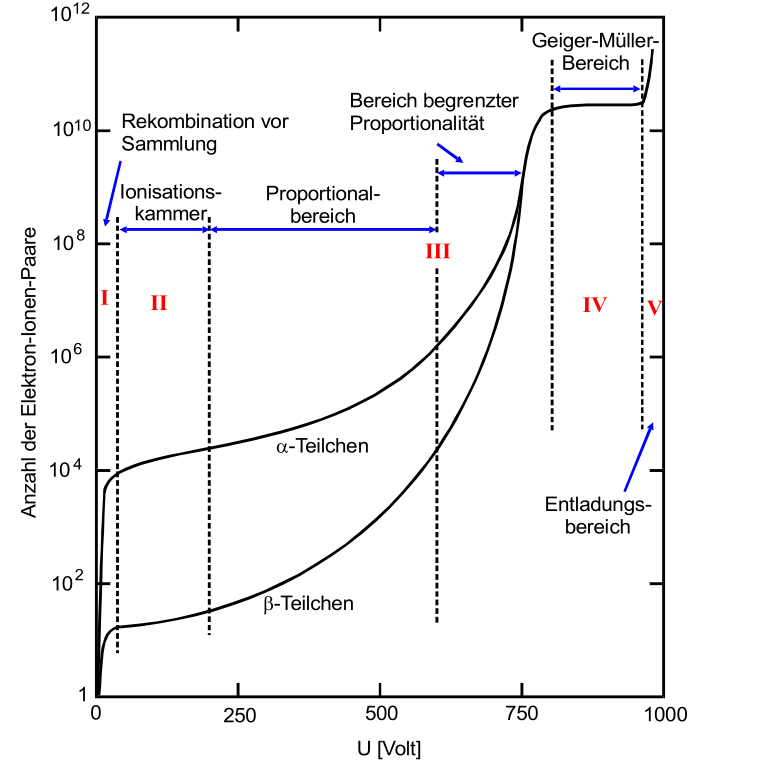
\includegraphics[width=\textwidth]{Bereiche.png}
  \caption{Die verschiedenen Bereiche im Bezug auf die angelegte Betriebsspannung.}
  \label{fig:Bereiche}
\end{figure}

\subsection{Einfluss der positiven Ionen}

Die frei gesetzten positiven Ionen bauen mit der Zeit im Zählrohr eine positive
Raumladung auf, welche einige Störeffekte hervorruft. Einerseits wird die
Feldstärke zwischenzeitlich so stark gesenkt, dass eintreffende Teilchen vom
Zählrohr nicht mehr registriert werden. Diesen Zeitraum nennt man auch Totzeit $T$.

Nach Auflösen bzw. Abwandern der positiven Raumladung wird stufenweise wieder eine
Lawinenbildung möglich, bis nach vollständiger Neutralisierung der Ionen nach der
Erhohlungszeit $T_E$ wieder Ladungsimpulse in ihrer ursprünglichen Höhe erreicht
werden.

Ein weiterer Störeffekt sind die Nachentladung. Diese entstehen wenn im Zählrohrmantel
auftreffende Ionen Elektronen aus der Metalloberfläche freisetzen und so mehrere
zeitlich versetzte Ausgangsimpulse erzeugt werden. Dieser Effekt ist höchst unerwünscht,
da er das Auftreffen von ionisierten teilchen vortäuscht, kann aber durch die anfangs
erwähnten Alkoholdämpfe im Zählrohr reduziert werden. Die frei werdende Energie
bei Stößen führt hier nicht zur Emission eines Elektrons sonder regt lediglich
die Schwingung eines vielatomigen Alkoholmoleküls an.

\subsection{Charakteristik des Zählrohrs}

Die Charakteristik eines Zählrohrs erhält man, wenn man die registrierte Teilchenzahl
N gegen die angelegte Spannung bei konstanter Strahlungsintensität aufträgt.

\begin{figure}
  \centering
  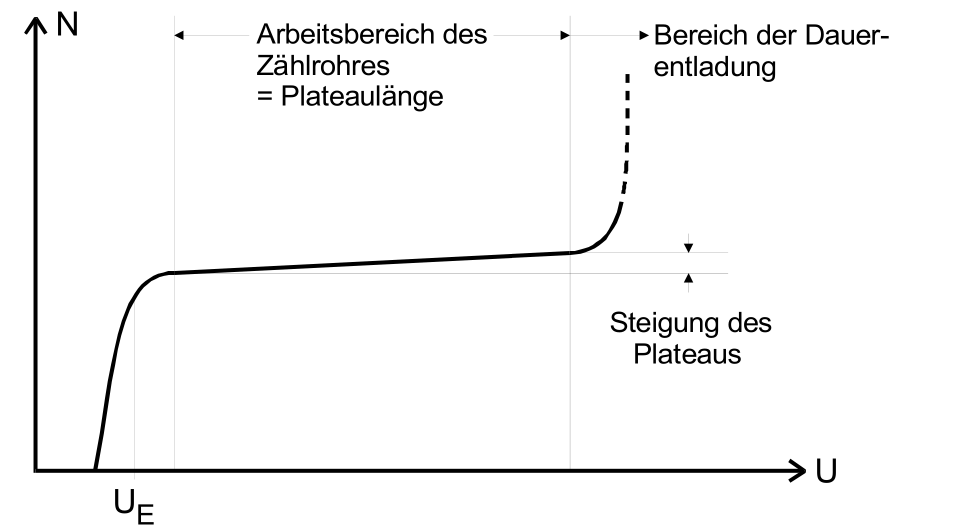
\includegraphics[width=\textwidth]{Charakteristik.png}
  \caption{Zählrohrcharakteristik bei konstanter Strahlungsintensität.}
  \label{fig:Charakteristik}
\end{figure}

Der lineare Teil der in Abb. \ref{fig:Charakteristik} zu sehenden Kurve heißt
Plateau. Durch Betrachtung der Plateausteigung sowie Spannungsmäßigen Ausdehnung
lässt sich eine Aussage über die Qualität des verwendeten Zählrohrs treffen, da
im Idealfall die Steigung null sein sollte und die Ausdehnung möglichst groß.
Aufgrund der Nachentladungen wird jedoch eine geringe Zunahme von N erkennbar sein.
Bei zu hoher Spannung wird die Zahl der Nachentladungen so groß, dass durch
selbstständige Gasentladungen das Zählrohr schnell zerstört wird (siehe auch Bereich
V in Abb. \ref{fig:Bereiche}).

\subsection{Ansprechvermögen des Zählrohrs}

Unter dem Ansprechvermögen versteht man die Wahrscheinlichkeit, dass ein in den
Detektro einfallendes Teilchen im Zählrohr nachgewiesen wird. Das Ansprechvermögen
für geladene teilchen wie $\alpha$- und $\beta$-Teilchen ist nahezu bei 100 \%.
Jedoch werden sie im metallischen Zählrohrmantel vollständig absorbiert. Um das
Zählrohr dennoch abschließen zu könne, wird bei den Endfensterzählrohren an der
Stirnseite eine Mylar-Folie angebracht, welche aus Atomen niedriger Ordnungszahl
besteht. Diese Folie kann selbst von $\alpha$-Teilchen durchdrungen werden und
wölbt sich aufgrund des Unterdruckes leicht nach Innen (Abb. \ref{fig:Geiger}).

Das Ansprechvermögen von Photonen ist aufgrund ihrer fehlenden Ladung äußerst
gering sodass eine Messung mit einem Geiger-Müller-Zählrohr lediglich bei
sehr hoher $\gamma$-Intensität sinnvoll ist.

\newpage

\section{Aufbau und Durchführung}

\begin{figure}
  \centering
  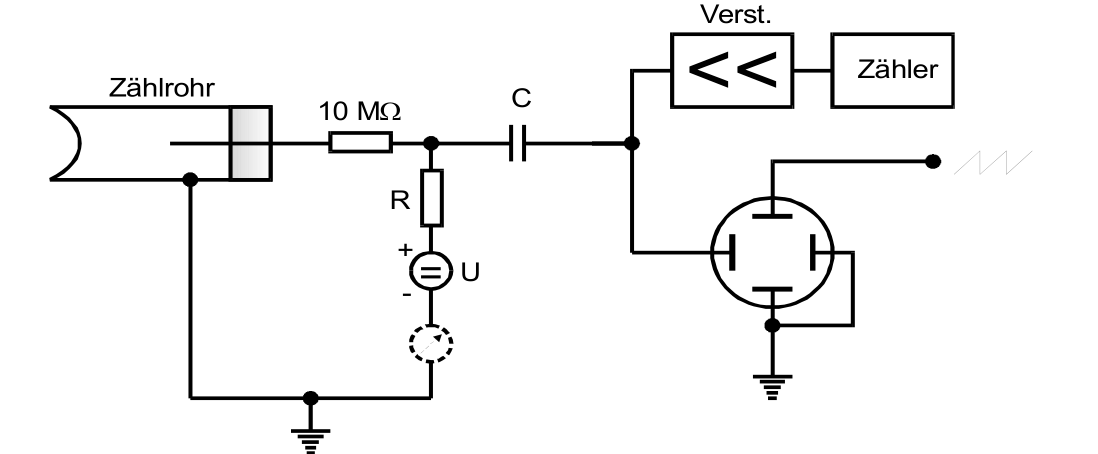
\includegraphics[width=\textwidth]{Aufbau.png}
  \caption{Aufbau der verwendeten Messapparatur.}
  \label{fig:Aufbau}
\end{figure}

Bei den folgenden Experimenten wird ein Aufbau gemäß Abbildung \ref{fig:Aufbau}
verwendet. Dabei fließt die auf dem Zähldraht gesammelten Ladung Q fließt über
den Widerstand R ab. Der entstehende Spannungsimpuls wird über einen Kondensator
ausgekoppelt, im Verstärker vergrößert und im Zahlgerät registriert oder auf einem
Oszilloskop sichtbar gemacht.

Im ersten Teil der Experimentes wird bei einer Probe die Abhängigkeit von gemessener
Teilchenzahl und Ionisierungstrom von der angelegten Spannung gemessen. Dafür wird
am Anfang eine Spannung von 300 V angelegt, die dann in 10 V Schritten bis auf 700 V
erhöht wird. Dabei werden nach jedem Schritt der Ionisierungsstrom sowie die in einem
Zeitintervall von $t=60 \, \su{s}$ auftreffenden Teilchen notiert.

Im nächsten Teil des Experimentes werden auf dem Oszilloskop die Totzeit und die
Erhohlungszeit ausgemessen bei einer Spannung von $U = 450 \, \su{V}$. Zudem werden
die Nachentladungen beobachtet.

Zum Abschluss wurde mit dem Zählrohr noch die eintreffende Teilchenzahl der
Probe $N_1$, der Proben $N_1$ und $N_2$ kombiniert sowie der Probe $N_2$ alleine
bei einer Spannung von $U = 450 \, \su{V}$ gemessen. Da jedoch keiner vernünftigen
Werte gemessen werden konnten, wird in der Auswertung auf die Ergebnisse der
Gruppe Stefan Grisard und Steven Becker zurückgegriffen.

\end{document}
